\documentclass[trackchanges]{aastex7}

\usepackage{graphicx}
\usepackage{amsmath}
\usepackage[caption=false]{subfig}
\submitjournal{Physics 212 at Harvard University}

\begin{document}

\title{Generating Mock Galaxy Catalogs}

\author[0009-0009-7258-1637]{Carl Audric Guia}
\email[show]{cgguia@college.harvard.edu}  
\affiliation{Harvard University, Cambridge, MA 02138, USA}

\begin{abstract}
    Mock galaxy catalogs are important in understanding the large scale structure of the universe and forecasting cosmological surveys.
    In this project, mock catalogs are constructed via forward modeling that begins with the linear power spectra generated by \texttt{CLASS}.
    The pipeline progresses through Gaussian field generation, bias expansion with stochastic noise, and perturbative predictions from \texttt{CLASS-PT}.
    Two cosmological models are considered: Planck \(\Lambda\)CDM and a \( w_0w_a \) dark energy model motivated by DESI DR2 forecasts.
    The result is then compared with theoretical predictions from \texttt{CLASS-PT} to ensure consistency.
    In the perturbative framework, the nonlinear corrections from \( P_{\text{1-loop, SPT}} \) are disabled.
    The simulated and theoretical power spectra of the galaxy fields exhibit consistent trends in redshift evolution and amplitude.
    In the $w_0 w_a$ model, suppression at low $k$ is observed across simulation and theory.
    This validates the forward-modeling pipeline of mock galaxy catalogs and supports its use in future work.
    More quantitative comparisons with perturbation theory and cosmological inference via \texttt{MCMC} are recommended.
    \end{abstract}
\keywords{\uat{Large-scale structure of the universe}{902} --- \uat{Cosmological perturbation theory}{341} --- \uat{Density parameters}{372} --- \uat{Galaxy formation}{595}}
\section{Introduction} \label{sec:intro}
The large-scale distribution of galaxies is central to cosmology. 
Galaxy surveys provide a window into the underlying matter field, and since galaxies are biased tracers of this structure, their distribution is shaped by a complex interplay of gravitational evolution and cosmological parameters. 
In bridging the gap between the initial matter field and the observed galaxy density today, mock galaxy catalogs play a critical role. 
They enable detailed tests of bias models, shot noise, and cosmic variance under controlled conditions, and they can validate pipelines in cosmological inference. 

This project constructs mock galaxy catalogs using a forward-modeling approach based on field-level perturbation theory. 
Two cosmological models are considered: Planck \(\Lambda\)CDM \citep{Planck2020} and a \( w_0w_a \) dark energy model motivated by DESI DR2 forecasts \citep{DESI2025}.
To isolate the potential effects of evolving dark energy on structure formation, the background cosmological parameters are fixed to the Planck 2018 \(\Lambda\)CDM best-fit values for both models.
This way, any differences in the power spectra are solely from the time-dependent dark energy equation of state in the \( w_0w_a \) model.

Starting from linear power spectra generated using \texttt{CLASS} \citep{CLASS2011}, Gaussian fields are sampled on a grid, and bias expansion is implemented to generate galaxy fields. 
The bias expansion includes linear, quadratic, and tidal terms, as well as a stochastic noise component \citep{Schmittfull2019}.
For both cosmological models, the tracer number density is fixed at \( \bar{n} = 10^{-3} \, h^3/\mathrm{Mpc}^3 \), which is the constraint for the Bright Galaxy Survey (BGS) as found by the \citet{DESI2025} forecasts.
Similarly consistent with \citet{DESI2016} and \citet{Chen2021} are the chosen bias parameters \( b_1 = 1.2 \), \( b_2 = -0.405 \), and \( b_{G_2} = -0.127 \). 

After computing the power spectra of the mock galaxy fields, the results are compared across redshift and cosmological models, as well as against theoretical predictions from \texttt{CLASS-PT} \citep{CLASSPT2020}, a perturbative Boltzmann code that includes 1-loop corrections. 
For consistency, the comparison is restricted to non-loop bias.

\section{Methods} \label{sec:methods}
\subsection{Overview of the Simulation Pipeline} \label{sec:pipeline_overview}

The pipeline automates the process of generating simulation outputs from theory using a sequence of Python scripts. It includes the following stages:

\begin{enumerate}
    \item Defining the fiducial cosmologies in the YAML files grounded in Planck 2018 and DESI 2025 forecasts.
    \item Generating linear matter power spectra at multiple redshifts using the \texttt{CLASS} Boltzmann solver.
    \item Constructing Gaussian initial conditions on a 3D grid by sampling $P(k)$ via FFT.
    \item Applying galaxy bias expansion to generate mock galaxy fields with shot noise.
    \item Computing power spectra for the Gaussian and galaxy fields binned in logarithmic $k$-space.
    \item Generating \texttt{CLASS-PT} predictions to validate simulation outputs.
\end{enumerate}


\subsection{Power Spectrum Generation with CLASS} \label{sec:class_yaml}

To compute the linear matter power spectrum \( P(k) \), the public Boltzmann solver \texttt{CLASS} \citep{CLASS2011} was used. 
It accepts cosmological parameters defined via YAML. 
For the Planck \(\Lambda\)CDM model, the parameters \( H_0 = 67.36 \), \( \Omega_b h^2 = 0.02237 \), \( \Omega_c h^2 = 0.1200 \) and one massive neutrino species (\( N_{\rm ncdm} = 1 \), \( m_{\rm ncdm} = 0.06 \)) were taken from the \citet{Planck2020}. 
For the \( w_0w_a \) model, the same background parameters were used to isolate the impact of dynamical dark energy on structure growth except for
\( w_0 = -0.838 \), \( w_a = -0.62 \), and \( \Omega_{\rm fld} = 0.6847 \) constrained by the \citet{DESI2025}. 

To ensure numerical stability in the phantom regime, the Parameterized Post-Friedmann (PPF) framework was activated for the dynamical dark energy model.
CLASS outputs $P(k)$ at redshifts $z = 0, 0.5, 1, 2, 3$ as two-column text files. 
These spectra serve as the input for generating the Gaussian field.

\subsection{Generating the Gaussian Field}

The Gaussian field is sampled in Fourier space on a \( 256^3 \) grid in a \( 1000 \, h^{-1} \mathrm{Mpc} \) box. Each $k$-mode is drawn as a complex Gaussian variable scaled by:
\begin{equation}
\delta(\vec{k}) = \left[ \mathcal{N}(0,1) + i \mathcal{N}(0,1) \right] \cdot \sqrt{\frac{P(k)}{2}}
\end{equation}
where $P(k) = \langle | \delta(k) |^2 \rangle = 2 \sigma^2$.
An inverse FFT with forward normalization brings the field into real space. 
The result is a mean-zero field with variance changing with the evolving redshift.


\subsection{Bias Expansion and Galaxy Field Construction}

To convert the Gaussian field into a mock galaxy field, the bias expansion by \citet{Schmittfull2019} is adopted:
\begin{equation}
\delta_h(\vec{x}) = b_1 \tilde{\delta}_1 + b_2 (\tilde{\delta}_1^2 - \langle \tilde{\delta}_1^2 \rangle) + b_{G_2} \tilde{G}_2 + \epsilon
\end{equation}
Here, $\tilde{\delta}_1(\vec{x}) = \delta_1(\vec{q} + \vec{\psi_1}(\vec{q}))$ is the displaced Gaussian field via the Zel'dovich approximation at first order. 
$\tilde{G}_2$, the tidal field operator, is implemented as follows:
\begin{equation}
    G_2 (\vec{q}) \equiv \left[\frac{\partial_i \partial_j}{\partial^2} \delta_1 (\vec{q})\right]^2 - \delta_1^2 (\vec{q})
\end{equation}
Lastly, $\epsilon(\vec{x}) \sim  \mathcal{N}\left(0, \frac{1}{\bar{n} V}\right)$ is the shot noise which models stochasticity. 
$V$ is the volume of the grid cell for proper scaling, and the mean number density $\bar{n} = 10^{-3} \, h^3/\mathrm{Mpc}^3$ is chosen consistent with the \citet{DESI2025} BGS samples. 
The shot noise adds a flat noise component to the galaxy power spectrum.
The operators are shifted to Eulerian space using cloud-in-cell interpolation, which is also used by \citet{Schmittfull2019}.

The bias parameters are fixed across redshifts and cosmologies as:
\begin{align}
b_1 = 1.2, \quad b_2 = -0.405, \quad b_{G_2} = -0.127
\end{align}
These are motivated by \citet{DESI2016} BGS forecasts and simulation-based fits by \citet{Chen2021}.


\subsection{Power Spectrum Computation and Binning}

To compute the power spectrum of the Gaussian and galaxy fields, FFT of the real-space density field was performed  using \texttt{numpy.fft.fftn}, again with forward normalization to ensure consistency with the input power spectrum. 
The resulting Fourier-space grid includes modes up to the Nyquist frequency, which is defined as
\[
k_{\rm Nyq} = \frac{\pi}{\Delta x} = \frac{\pi \cdot n_{\rm grid}}{L}
\]
$k_{\rm Nyq}$ represents the smallest wavelength that can be unambiguously sampled on the discrete grid, a foundational result of the Shannon Sampling Theorem \citep{Shannon1949}.

The power spectrum is computed from the squared Fourier amplitudes and then binned into logarithmically spaced \( k \)-bins up to \( k_{\rm Nyq} \). 
This ensures that all modes contributing to the power spectrum are below the aliasing threshold, and the resulting \( P(k) \) is not undersampled.
Up to a factor of $2\pi$, the power spectrum is
\begin{equation}
P(k) = |\delta_k|^2 \cdot V
\end{equation}
The Planck $\Lambda$CDM universe is binned into 8 intervals, while the $w_0 w_a$ model is binned into 7 to balance resolution with statistical noise at low and high $k$.

\subsection{CLASS-PT Prediction and Parameter Setup}

\texttt{CLASS-PT} \citep{CLASSPT2020} was used to generate theoretical galaxy power spectra. It is a perturbative extension of \texttt{CLASS} that includes 1-loop perturbation theory and bias modeling. 
For consistency with the mock galaxy field pipeline, non-linear corrections are exclused by setting:
\begin{equation}
cs_0 = cs_2 = cs_4 = b_{\Gamma_3} = b_4 = 0
\end{equation}
This removes $P_{\rm 1-loop, SPT}$ from the total spectrum as described in Equation (2.10) of \citet{CLASSPT2020}. 
The bias parameters $b_1, b_2,$ and $b_{G2}$ in the mock galaxy field are retained to allow for direct $P_{gg}(k)$ comparisons with CLASS-PT outputs across all redshifts and cosmologies.

\section{Results} \label{sec:results}

\subsection{Field-Level Statistics}

The variance of the Gaussian fields decreases with redshift due to suppressed growth of structure at early times.
The galaxy fields, on the other hand, exhibit higher variance across all redshifts as shown in Table~\ref{tab:field_variance}. 
This amplification is consistent with the inclusion of linear and nonlinear bias terms in the expansion. 
Figure~\ref{fig:galaxy_slices_stacked} also aligns with this amplification by showing the enhanced density contrast of the galaxy fields.
The variance remains relatively flat from $z = 0$ to $z = 3$, reflecting the dominant contribution of biasing and shot noise, but the trend is still decreasing as anticipated.
Also, the variances between the two models are very similar, an observation supported by the nearly identical power spectra below. 

\begin{table}[ht]
    \centering
    \caption{Variance of Gaussian and galaxy fields across redshift for Planck \(\Lambda\)CDM and \( w_0w_a \) cosmological models. Each value corresponds to the variance of the field computed on a \( 256^3 \) grid in a \( 1000 \, h^{-1}\mathrm{Mpc} \) box.}
    \label{tab:field_variance}
    \begin{tabular}{llccccc}
    \hline
    \textbf{Model} & \textbf{Field} & \( z = 0.0 \) & \( z = 0.5 \) & \( z = 1.0 \) & \( z = 2.0 \) & \( z = 3.0 \) \\
    \hline
    Planck \(\Lambda\)CDM & Gaussian & 2.40101 & 1.42006 & 0.88660 & 0.42030 & 0.24007 \\
    Planck \(\Lambda\)CDM & Galaxy   & 22.07993 & 19.44727 & 18.29369 & 17.44254 & 17.14807 \\
    \( w_0w_a \)          & Gaussian & 2.42002 & 1.44392 & 0.90267 & 0.42381 & 0.24199 \\
    \( w_0w_a \)          & Galaxy   & 22.11306 & 19.50880 & 18.33609 & 17.43391 & 17.14452 \\
    \hline
    \end{tabular}
\end{table}

\begin{figure}[ht]
    \centering
    \subfloat[Planck \(\Lambda\)CDM]{%
        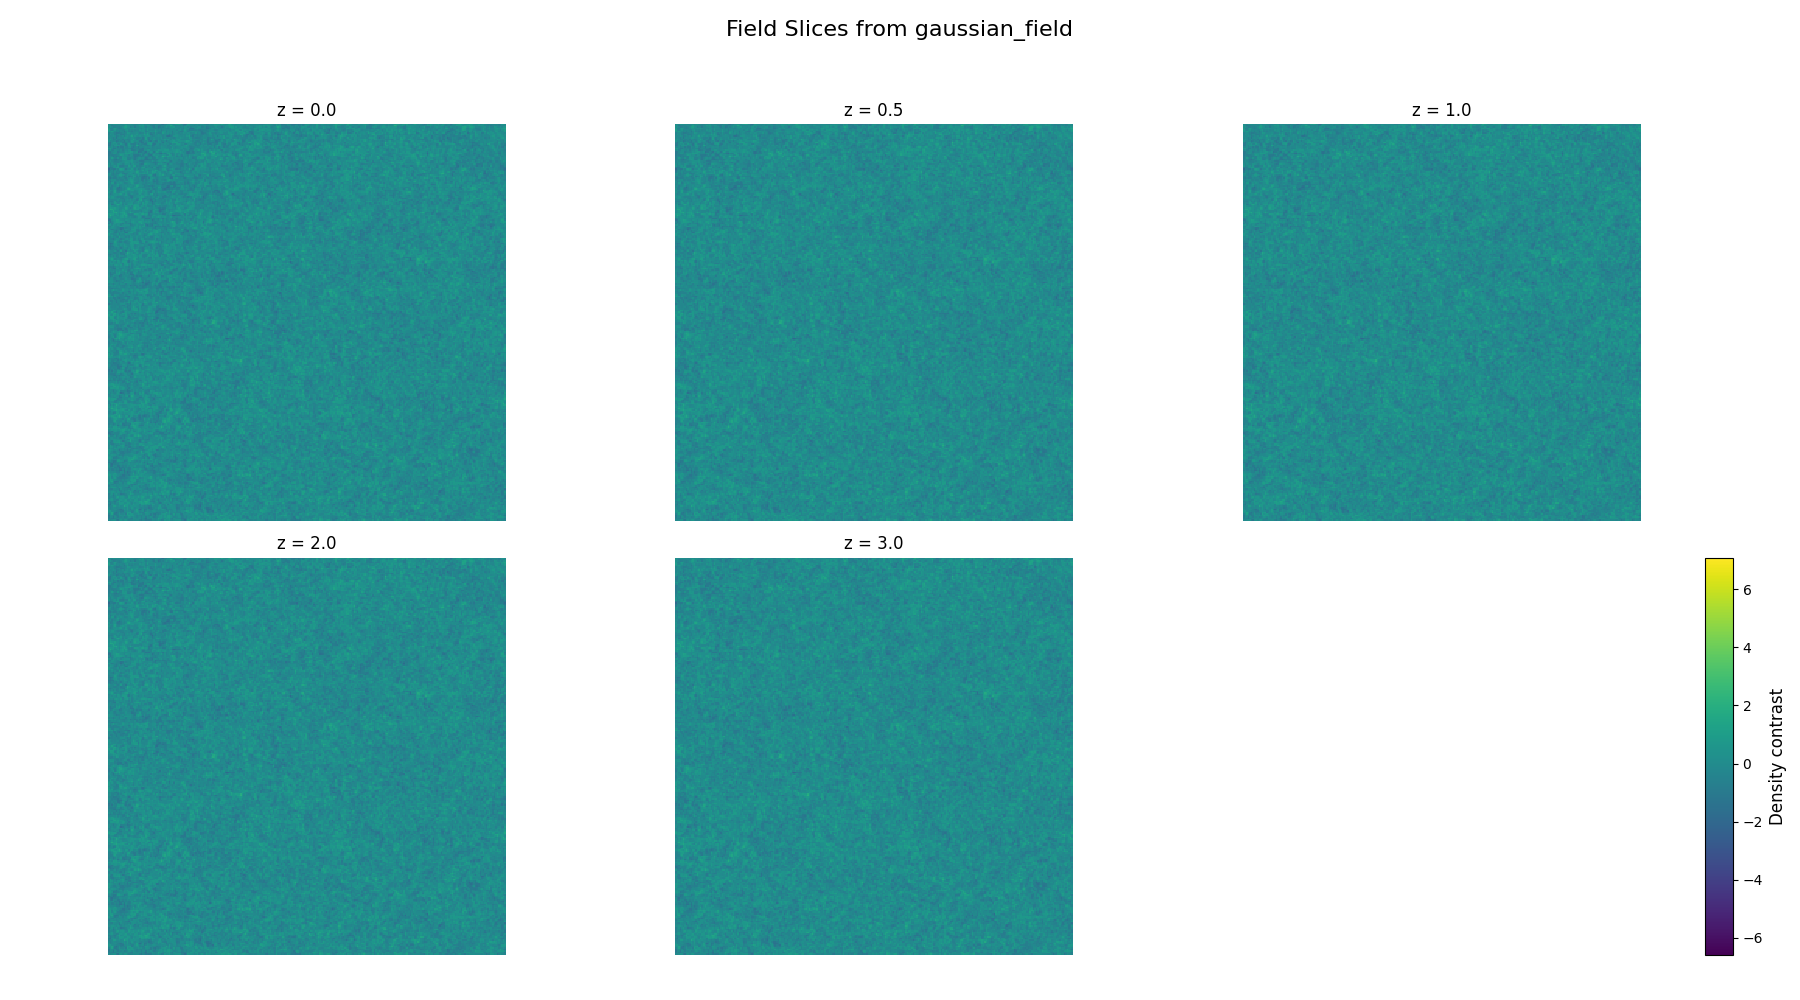
\includegraphics[width=0.85\linewidth]{../output/planck_lcdm/gaussian_field/field_grid.png}
        \label{fig:gaussian_slices1}
    }\\[0.5em]
    \subfloat[\( w_0w_a \) model]{%
        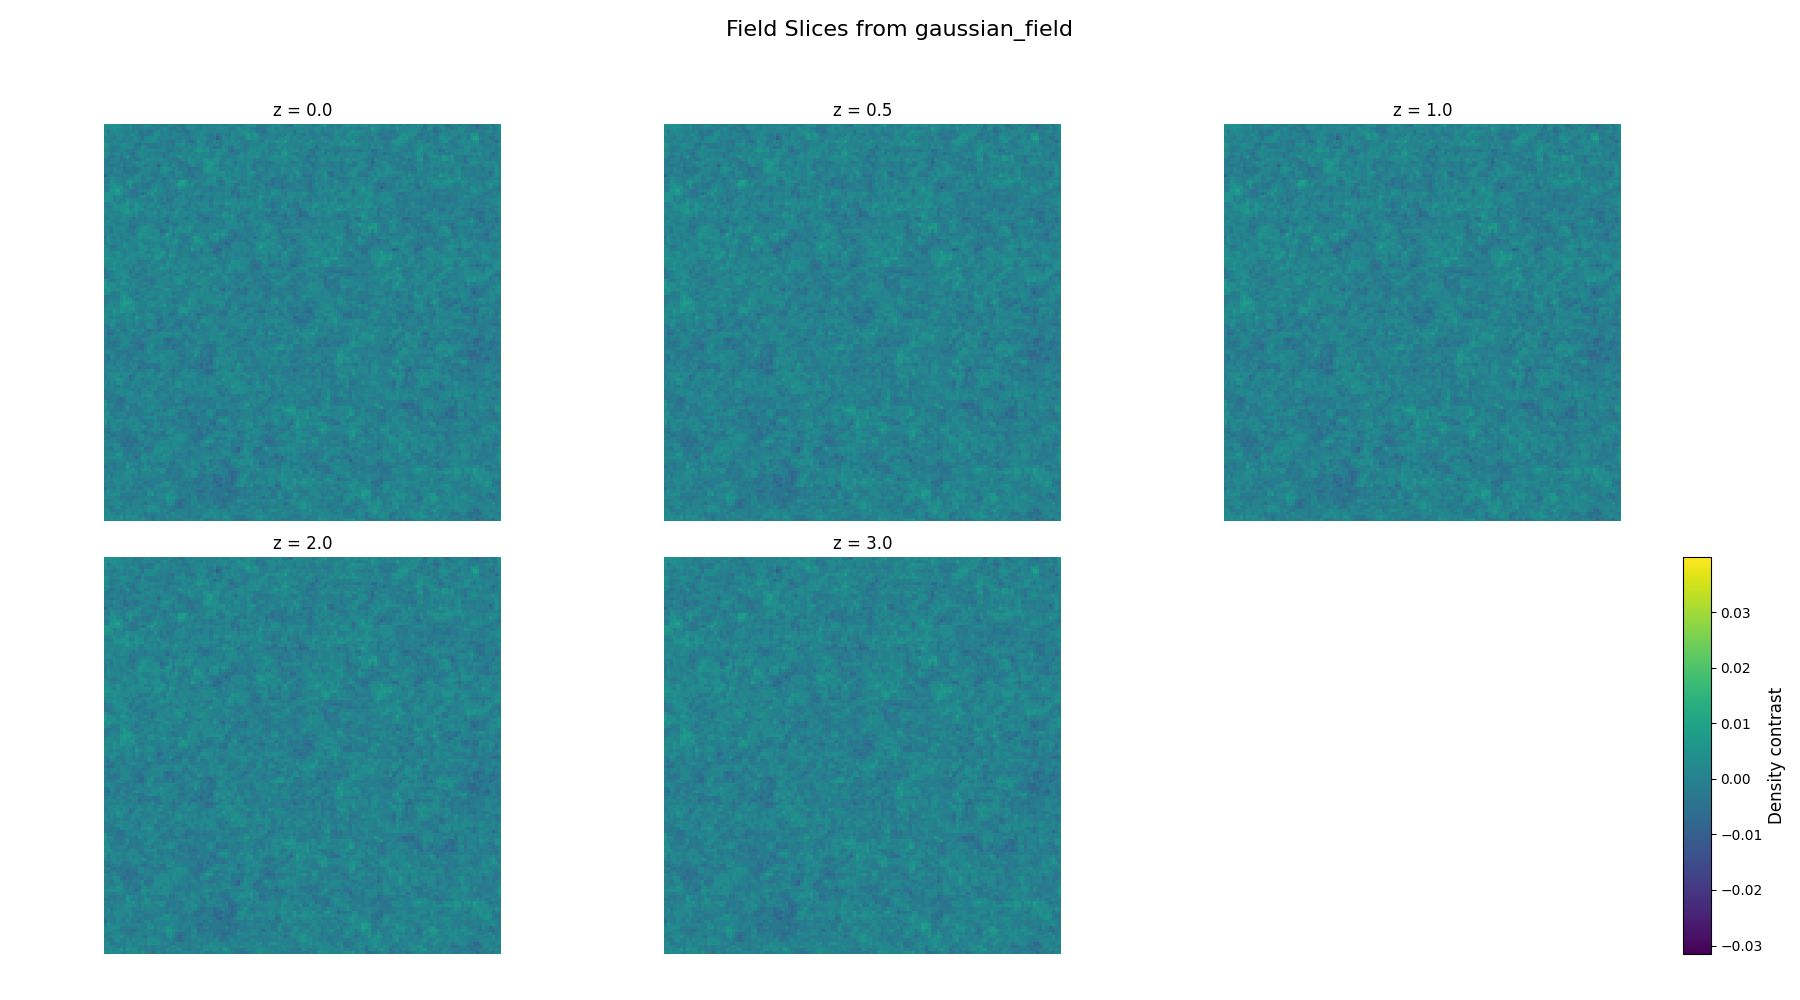
\includegraphics[width=0.85\linewidth]{../output/w0wa/gaussian_field/field_grid.png}
        \label{fig:gaussian_slices2}
    }
    \caption{Slices of the real-space Gaussian field \(\delta(x)\) for both cosmological models. Each field is generated from the linear power spectrum using a common grid and random seed.}
    \label{fig:gaussian_slices_stacked}
\end{figure}

\begin{figure}[ht]
    \centering
    \subfloat[Planck \(\Lambda\)CDM]{%
        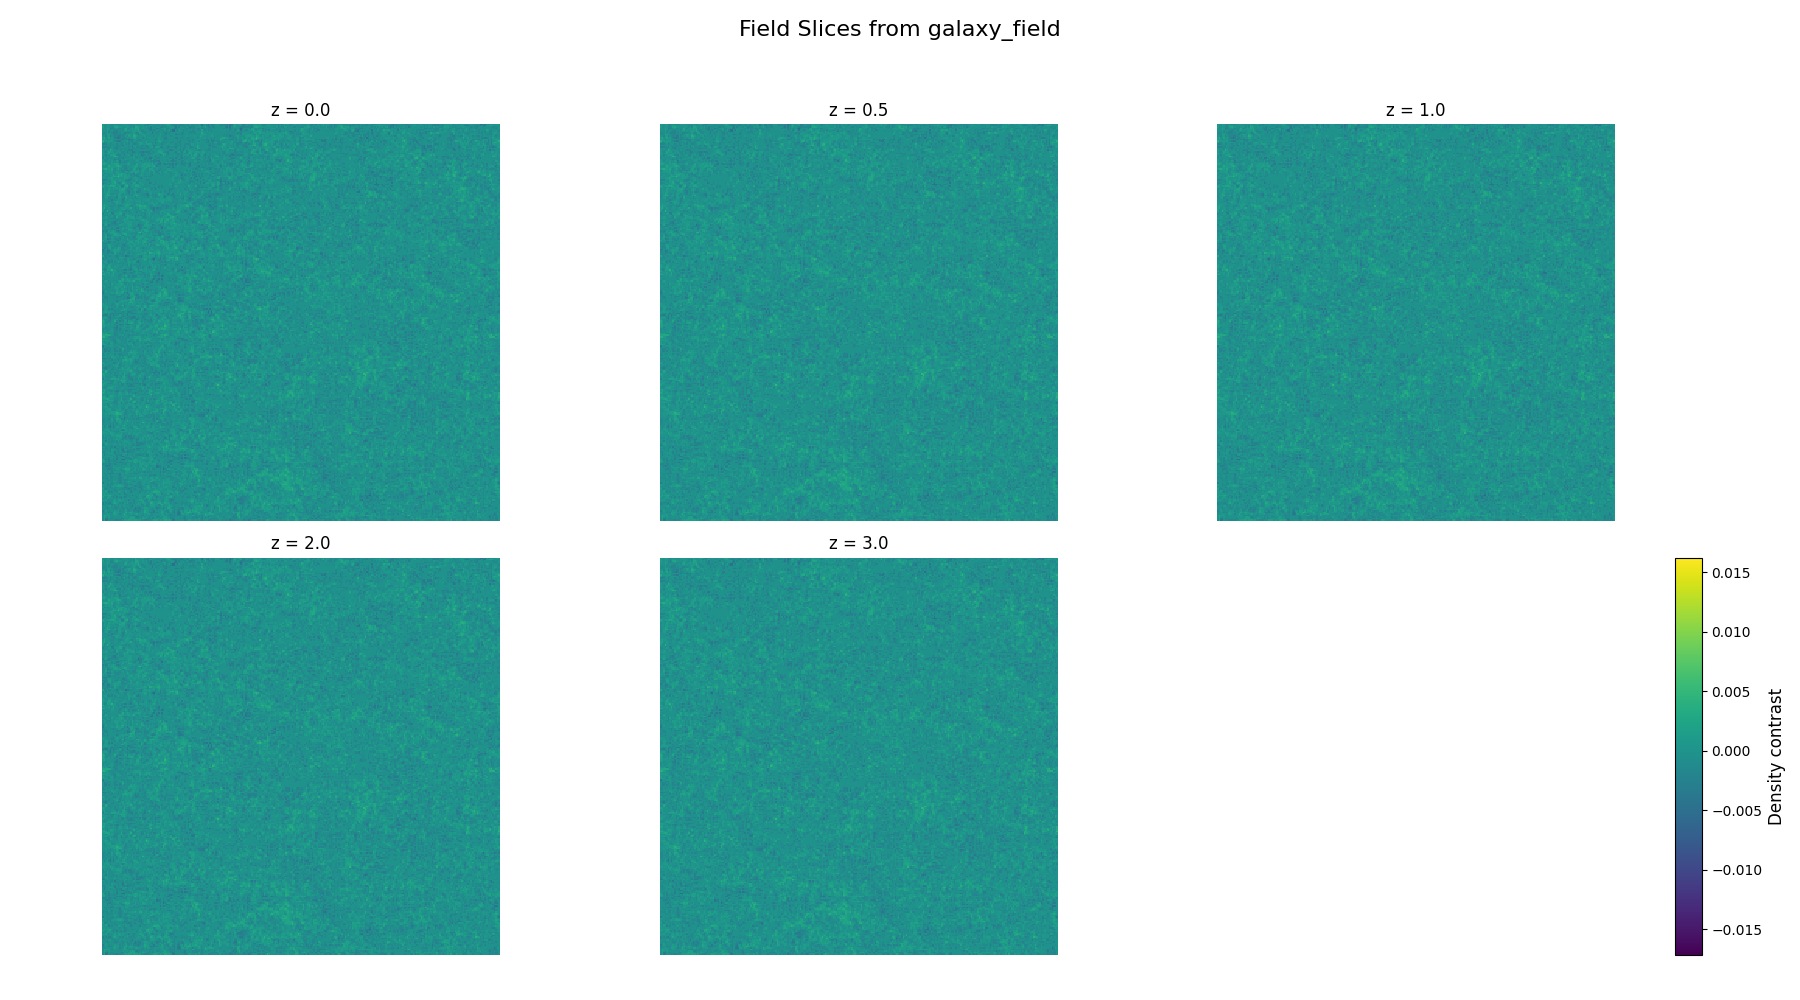
\includegraphics[width=0.85\linewidth]{../output/planck_lcdm/galaxy_field/field_grid.png}
        \label{fig:galaxy_slices1}
    }\\[0.5em]
    \subfloat[\( w_0w_a \) model]{%
        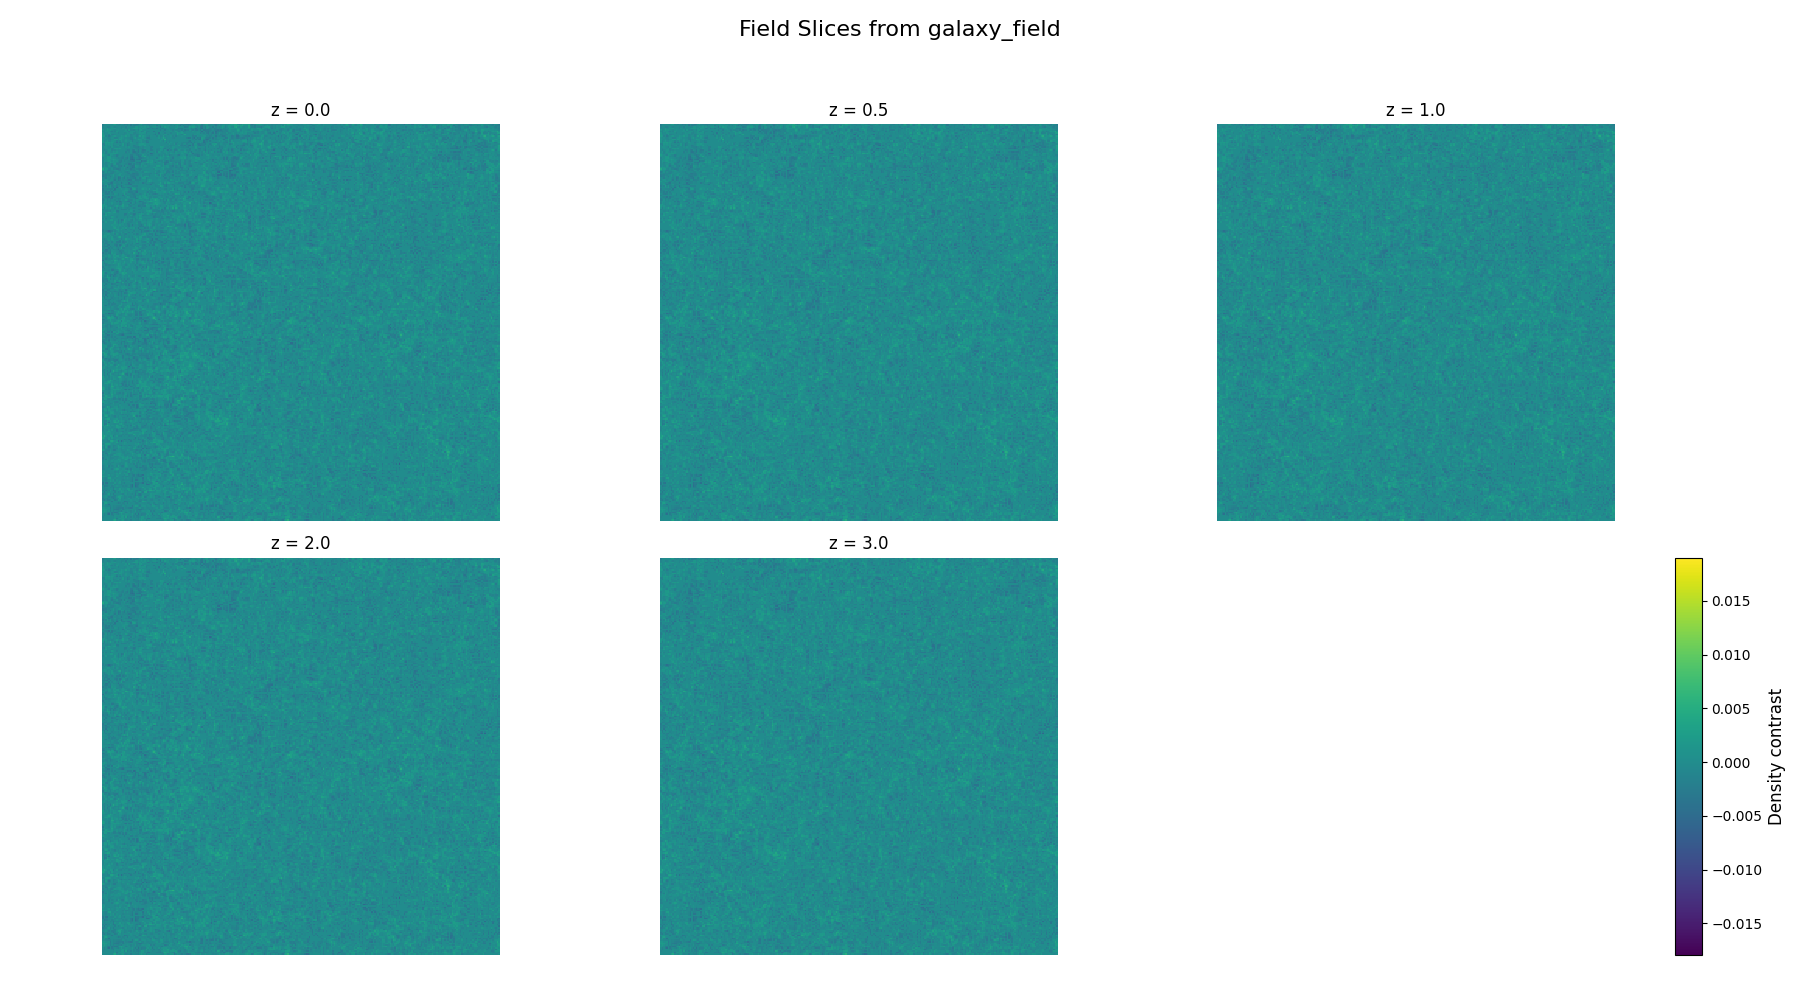
\includegraphics[width=0.85\linewidth]{../output/w0wa/galaxy_field/field_grid.png}
        \label{fig:galaxy_slices2}
    }
    \caption{Slices of the real-space galaxy field \(\delta_h(x)\) for both cosmological models, generated by applying the bias expansion and shot noise to the underlying Gaussian matter field.}
    \label{fig:galaxy_slices_stacked}
\end{figure}
\clearpage

\clearpage
\subsection{Mock Galaxy Power Spectra}

The \texttt{CLASS}-computed power spectra in Figure~\ref{fig:pk_class_side_by_side} show a consistent decline in amplitude with increasing redshift, reflecting the suppression of structure growth in early times. 
Small-amplitude oscillations are visible in the intermediate $k$-range, corresponding to baryon acoustic oscillations (BAOs) imprinted at recombination. 
The linear power spectra produced by \texttt{CLASS} are nearly indistinguishable between the two cosmologies across redshifts. 
This reflects the fact that early-time physics is identical between the two models. 
This result might hint at the insensitivity of the linear power spectrum to the dark energy equation of state.

Figure \ref{fig:pk_gaussian_side_by_side} displays the power spectra of the Gaussian density fields for the two cosmologies.
As expected, the amplitude of $P(k)$ declines with increasing redshift. 
The spectra from both models exhibit a similar shape consistent with Figure~\ref{fig:pk_class_side_by_side}. 
The BAO features appear somewhat jagged due to limited k-resolution from binning: with only 7–8 logarithmic bins used to reduce noise, individual BAO wiggles are not fully resolved.

Figure \ref{fig:pk_galaxy_side_by_side} shows the galaxy power spectra derived from the bias expansion applied to the Gaussian fields, incorporating both nonlinear bias terms and stochastic shot noise.
Compared to the Gaussian field spectra, the galaxy spectra exhibit an overall enhancement in amplitude particularly at low $k$.
This might be due to the contribution of the linear bias term $b_1^2$. 
A flat high-$k$ tail is visible in both cosmologies as expected from the stochastic noise $P_\epsilon(k) \sim 1/\bar{n}$ from $\epsilon(x)$. 
The amplitude of this tail matches $\bar{n} = 10^{-3} \, h^3/\mathrm{Mpc}^3$. 
These results validate the implementation of the bias expansion including stochastic noise.
\begin{figure*}[ht]
    \centering
    \subfloat[Planck \(\Lambda\)CDM]{%
        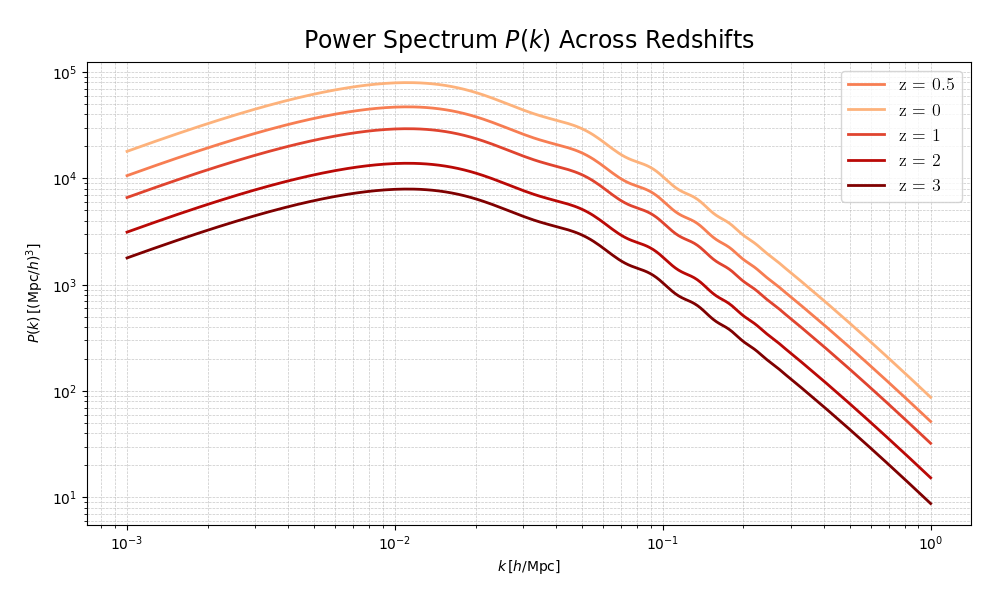
\includegraphics[width=0.48\linewidth]{../output/planck_lcdm/pk/pk_pk_multi_z.png}
        \label{fig:pk_class_lcdm_side}
    }
    \hfill
    \subfloat[\( w_0w_a \) model]{%
        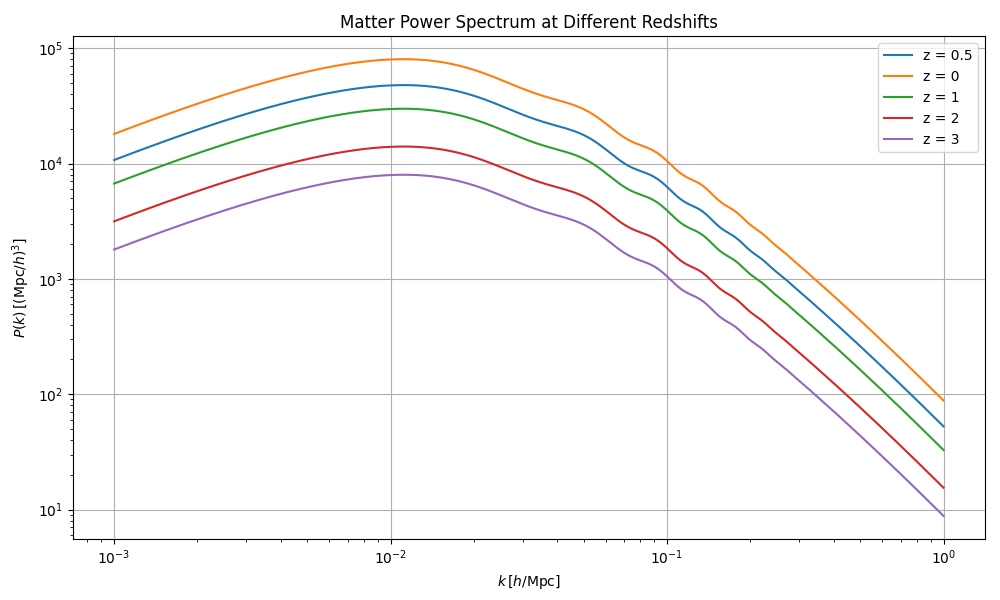
\includegraphics[width=0.48\linewidth]{../output/w0wa/pk/pk_pk_multi_z.png}
        \label{fig:pk_class_w0wa_side}
    }
    \caption{Comparison of CLASS power spectra between the two cosmological models at various redshifts.}
    \label{fig:pk_class_side_by_side}
\end{figure*}

\begin{figure*}[ht]
    \centering
    \subfloat[Planck \(\Lambda\)CDM]{%
        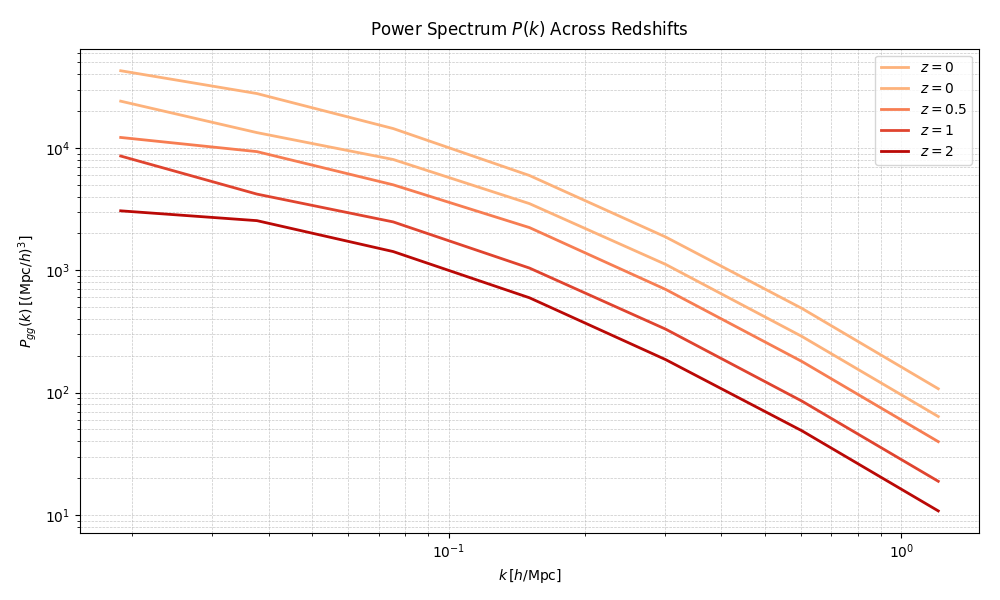
\includegraphics[width=0.48\linewidth]{../output/planck_lcdm/gaussian_field/field_power_spectrum.png}
        \label{fig:pk_gaussian_lcdm}
    }
    \hfill
    \subfloat[\( w_0w_a \) model]{%
        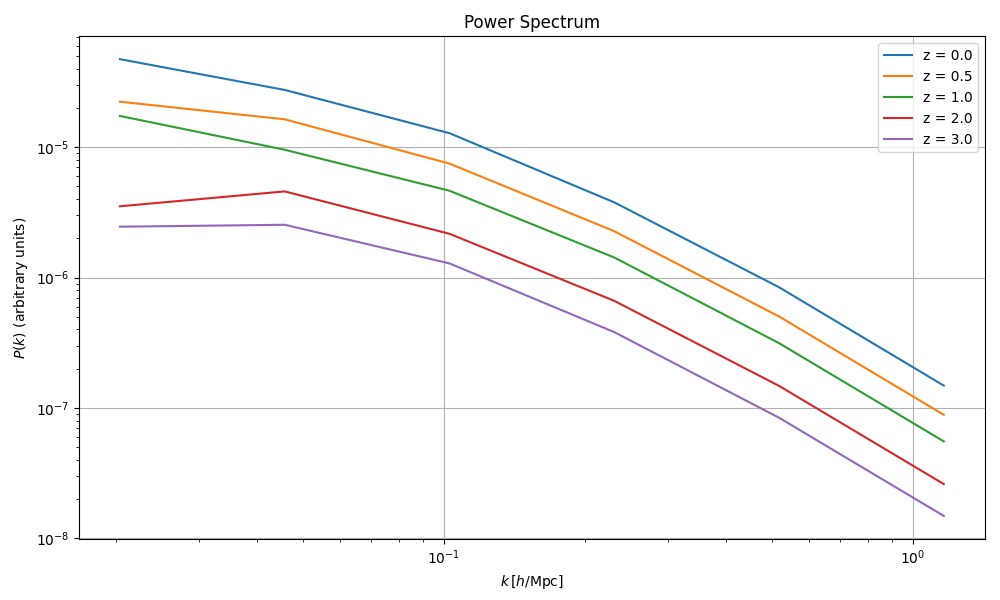
\includegraphics[width=0.48\linewidth]{../output/w0wa/gaussian_field/field_power_spectrum.png}
        \label{fig:pk_gaussian_w0wa}
    }
    \caption{Comparison of Gaussian field power spectra between the two cosmological models at various redshifts.}
    \label{fig:pk_gaussian_side_by_side}
\end{figure*}

\begin{figure*}[ht]
    \centering
    \subfloat[Planck \(\Lambda\)CDM]{%
        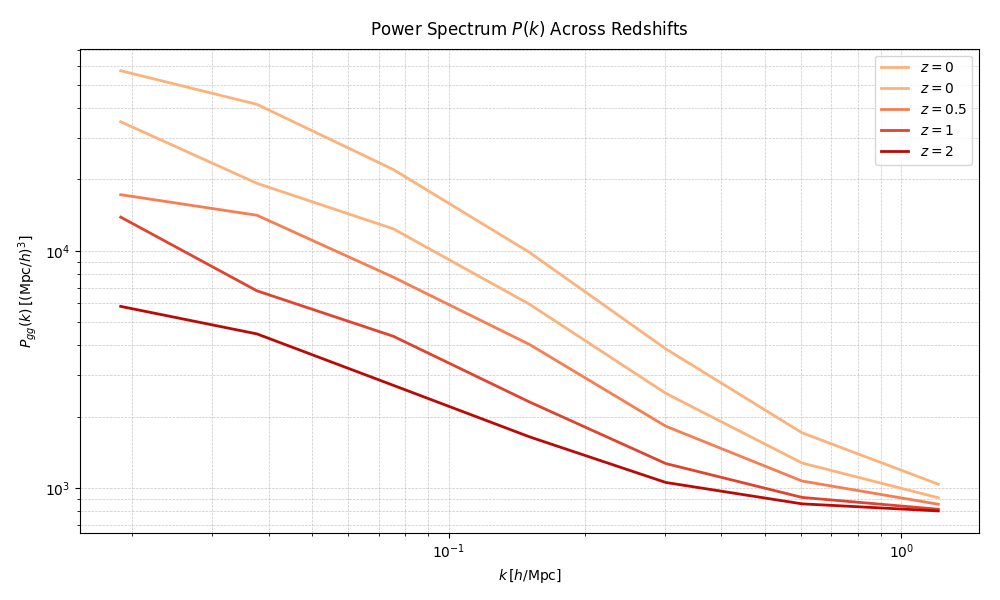
\includegraphics[width=0.48\linewidth]{../output/planck_lcdm/galaxy_field/field_power_spectrum.png}
        \label{fig:pk_galaxy_lcdm}
    }
    \hfill
    \subfloat[\( w_0w_a \) model]{%
        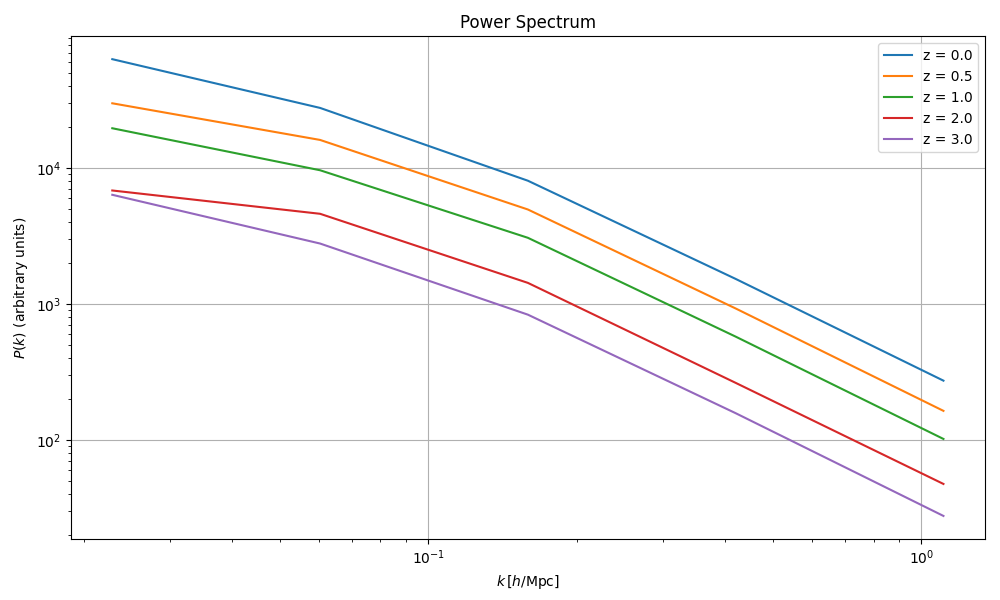
\includegraphics[width=0.48\linewidth]{../output/w0wa/galaxy_field/field_power_spectrum.png}
        \label{fig:pk_galaxy_w0wa}
    }
    \caption{Galaxy power spectra with biasing and shot noise for Planck \(\Lambda\)CDM and \( w_0w_a \) cosmologies across redshift. }
    \label{fig:pk_galaxy_side_by_side}
\end{figure*}

\subsection{Comparison with CLASS-PT}

Figure \ref{fig:pk_classpt_side_by_side} shows the galaxy power spectra predicted by \texttt{CLASS-PT} for both cosmologies.
With non-loop bias only, the overall shape and redshift evolution of these spectra resemble those of the mock galaxy fields in Figure \ref{fig:pk_galaxy_side_by_side} in the applicable $k$-domain.
As in the mock fields, the amplitude decreases with redshift. 
A flat high-$k$ tail is present as well, something that was not observed with only \texttt{CLASS}.
The similarity in structure and redshift trends between the simulations and \texttt{CLASS-PT} validates the consistency of the field-level bias expansion.
\begin{figure*}[ht]
    \centering
    \subfloat[Planck \(\Lambda\)CDM]{%
        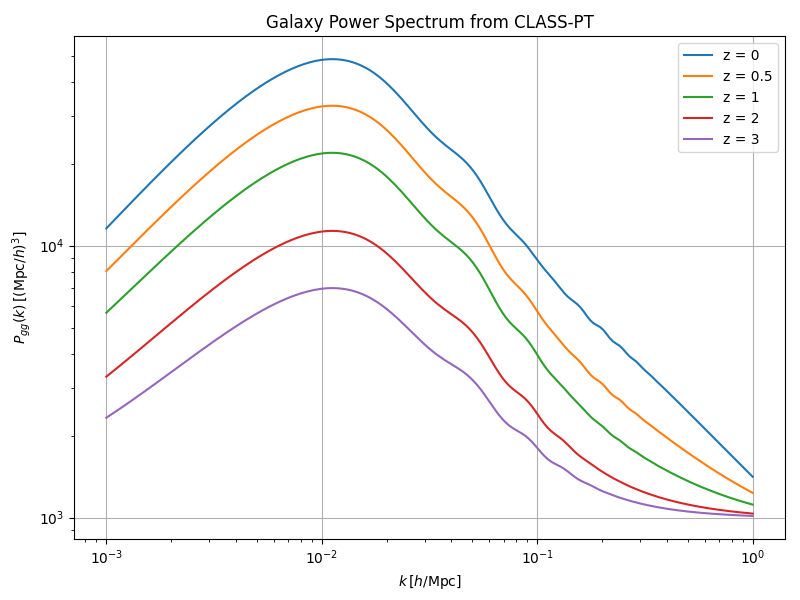
\includegraphics[width=0.48\linewidth]{../output/planck_lcdm/classpt/pk_planck_lcdm_classpt.png}
        \label{fig:pk_classpt_lcdm}
    }
    \hfill
    \subfloat[\( w_0w_a \) model]{%
        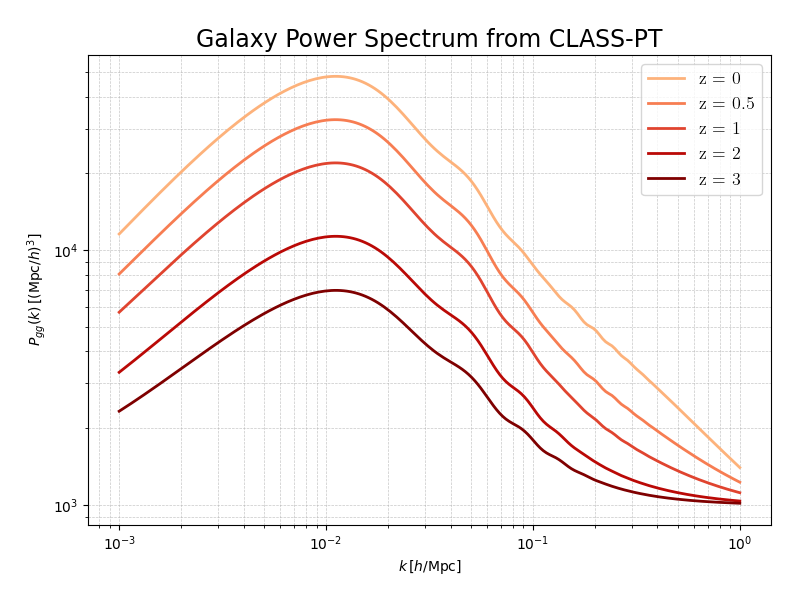
\includegraphics[width=0.48\linewidth]{../output/w0wa/classpt/pk_w0wa_classpt.png}
        \label{fig:pk_classpt_w0wa}
    }
    \caption{CLASS-PT predictions for the galaxy power spectrum with non-loop bias for both cosmological models.}
    \label{fig:pk_classpt_side_by_side}
\end{figure*}


\section{Recommendations} \label{sec:recommendations}

While the results show qualitative agreement with \texttt{CLASS-PT} predictions and highlight the effects of bias in structure growth, several natural extensions would bolster the robustness of this work.

\subsection{Quantitative Comparison with Perturbation Theory}

Future work could benefit from a more quantitative analysis. 
This includes computing the residuals and RMS fractional errors between the simulated and \texttt{CLASS-PT} power spectra across redshifts and scales. 
Such a comparison would clarify the parameter space where non-loop perturbation theory remains valid.

\subsection{Likelihood Construction and Cosmological Inference}

The outputs of the simulation can be treated as synthetic observations and compared to theoretical predictions from \texttt{CLASS-PT} using an \texttt{MCMC} sampler such as \texttt{Cobaya} or \texttt{emcee}. 
This would provide a consistency check: by treating \( b_1, b_2, b_{G_2} \) and \( c_s^2 \) as free parameters, one could test whether the input parameters can be recovered to generate the mock galaxy fields.

In principle, \( c_s^2 \) should be included in this analysis, even though it was set to zero in the present work. 
It accounts for small-scale nonlinear corrections from the nonlinear matter density and is related to the resolution of the simulated field. 
While it is justified to set \( c_s^2 = 0 \) when modeling only non-loop bias on linear Gaussian field, a more complete framework should account for this parameter to minimize systematic errors.

\subsection{Higher-Order Statistics}

The bispectrum and other higher-order statistics could be computed from the simulated fields. 
This would test whether the nonlinear bias model captures three-point correlations, which can be a probe of primordial non-Gaussianity $f_{\text{NL}}$.
Computing the bispectrum would also provide more insight into the effects of massive neutrinos at different scales.

\begin{acknowledgments}
    The author thanks Cora Dvorkin and Prish Chakraborty for their mentorship in this project.
\end{acknowledgments} 

\bibliography{ms}{}
\bibliographystyle{aasjournal}

\end{document}